\documentclass[12pt]{article} % Default font size is 12pt, it can be changed here

\usepackage{geometry} % Required to change the page size to A4
\geometry{a4paper} % Set the page size to be A4 as opposed to the default US Letter

\usepackage{graphicx} % Required for including pictures

\usepackage{float} % Allows putting an [H] in \begin{figure} to specify the exact location of the figure
\usepackage{wrapfig} % Allows in-line images such as the example fish picture

\usepackage[portuguese]{babel}
\usepackage[utf8]{inputenc}

\usepackage{lipsum} % Used for inserting dummy 'Lorem ipsum' text into the template

\linespread{1.2} % Line spacing

\graphicspath{{Pictures/}} % Specifies the directory where pictures are stored

\begin{document}
José Pereira (pg 27748), Marta Azevedo (pg27763), Tiago Brito (pg27724)

\section{Elevador} % Major section

Neste exercício, foi pedido para modelar um elevador autónomo que anda entre dois andares - {\it{Ground Floor}} e {\it{First Floor}}. As condições são as seguintes:
\begin{itemize}
\item O elevador pode parar no {\it{Ground Floor}} ou no {\it{First Floor}};
\item Quando o elevador chega a um dado piso, a sua porta abre automaticamente.
\item Leva 2 segundos a abrir a porta desde a sua chegada, mas a porta abre dentro de 5 segundos;
\item Os passageiros podem entrar assim que a porta abrir;
\item Os passageiros entram um por um e não há limite máximo de passageiros no elevador;
\item A porta fecha 4 segundos depois do último passageiro entrar;
\item Depois da porta fechar, o elevador espera 2 segundos e só então se desloca.
\end{itemize}

Para resolver este exercício, usámos 2 templates: {\it{Elevator}} e {\it{Door}}. 
\\

Foram necessários 5 canais de sincronização ({\it{open,close,up,down,enter}}), um relógio {\it{x}} que controla o tempo do elevador e uma variável {\it{waiting}} que significa o número de pessoas que está à espera para entrar no elevador.
\\
Sendo assim, o nossos autómatos temporais são:
\begin{center}
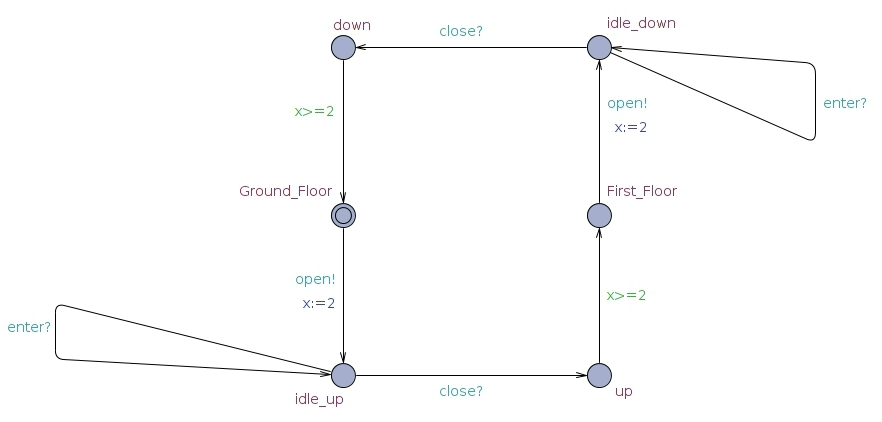
\includegraphics[scale=0.4]{elevator.jpg}
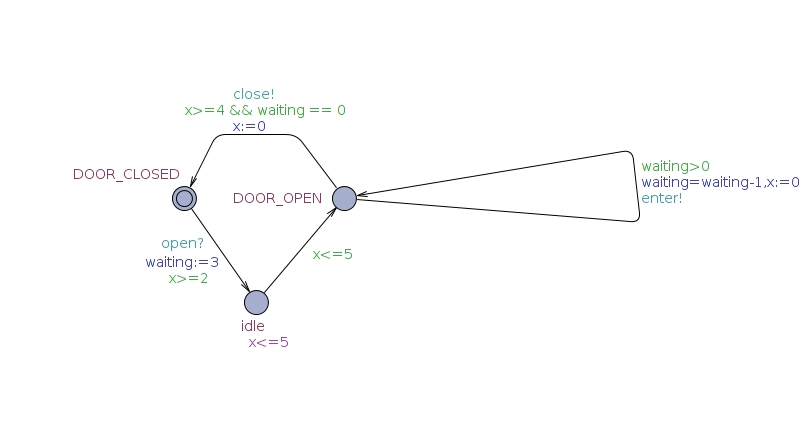
\includegraphics[scale=0.4]{door.jpg}
\end{center}


\section{QoS} 

Neste exercício, devemos modelar um {\it{stream channel}} tal que:
\begin{enumerate}
\item A {\it{Source}} envia mensagens a cada 50ms;
\item O {\it{Channel}} pode perder mensagens mas não mais que 20$\%$;
\item Se a mensagem não chegar ao {\it{Reciever}} em 90ms, é considerada perdida: {\it{lost}};
\item O {\it{Reciever}} recebe mensagens e demora 5ms a processá-las;
\item Se em 1 segundo (1000 ms) não chegarem 15 mensagens, é gerada uma mensagem de erro: {\it{error}}.
\end{enumerate}

Para resolver estes problemas, criamos 3 templates: {\it{Soucer}}, {\it{Worker}}, {\it{Source$\_$Worker}} e inserimos as seguintes especificações para solucionar os problemas acima mencionados:

\begin{enumerate}
\item No {\it{Source}}, o clock é reniciado e espera até chegar aos 50 ms para enviar a mensagem;
\item Há um contador para as mensagens enviadas (msgSend) e as que foram perdidas (msgLost) e também foi criado uma função chamada {\it{value()}}. Assim que as mensagens perdidas atingirem mais que 20$\%$ das mensagens enviadas, o autómato pára a sua execução;
\item Cada mensagem tem um relógio (solucionado através da introdução de um array de relógios). Quando o receiver recebe a mensagem, vê no respetivo  relógio se já passaram 90ms. Se já tiver passado, envia um sincronismo a avisar que essa mensagem foi perdida ({\it{lost!}}) ;
\item Existe um nodo no {\it{Reciever}} chamado {\it{Process}} que só avança quando o seu temporizador chegar a 5ms;
\item Há um contador geral e cada vez que atinge os 1000 ms (1 segundo), o {\it{Reciever}} vê quantas mensagens ja foram enviadas (msgSend), e se forem menos de 15 é diaparado um sincronismo {\it{error!}}.
\end{enumerate}

Para receber os sincronismos de falha ({\it{error, lost}}) e para receber o de sucesso ({\it{reply}}) existe o template {\it{Source$\_$Worker}}. No caso dos sincronismos de falha, renicia o autómato e no caso do 
{\it{reply}} incrementa o numero de mensagens enviadas com sucesso (msgOK) e renicia o autómato.



%----------------------------------------------------------------------------------------

\end{document}